\documentclass[journal,12pt,twocolumn]{IEEEtran}
%
\makeatletter
\makeatother
\usepackage{setspace}
\usepackage{gensymb}
\usepackage{xcolor}
\usepackage{caption}
%\usepackage{stackengine}
%\usepackage{subcaption}
%\doublespacing
\singlespacing



\usepackage{graphicx}
\graphicspath{ {./images}  }
%\usepackage{amssymb}
%\usepackage{relsize}
\usepackage[cmex10]{amsmath}
\usepackage{mathtools}
%\usepackage{amsthm}
\interdisplaylinepenalty=2500
%\savesymbol{iint}
%\usepackage{txfonts}
%\restoresymbol{TXF}{iint}
\usepackage{wasysym}
\usepackage{amsthm}
\usepackage{mathrsfs}
\usepackage{txfonts}
\usepackage{stfloats}
\usepackage{cite}
\usepackage{cases}
\usepackage{mathtools}
\usepackage{subfig}
\usepackage{enumerate}	
\usepackage{enumitem}
\usepackage{amsmath}
%\usepackage{xtab}
\usepackage{longtable}
\usepackage{multirow}
%\usepackage{algorithm}
%\usepackage{algpseudocode}
\usepackage{enumitem}
\usepackage{mathtools}
%\usepackage{iithtlc}
%\usepackage[framemethod=tikz]{mdframed}
\usepackage{listings}
\usepackage{listings}
    \usepackage[latin1]{inputenc}                                 %%
    \usepackage{color}                                            %%
    \usepackage{array}                                            %%
    \usepackage{longtable}                                        %%
    \usepackage{calc}                                             %%
    \usepackage{multirow}                                         %%
    \usepackage{hhline}                                           %%
    \usepackage{ifthen}                                           %%
  %optionally (for landscape tables embedded in another document): %%
    \usepackage{lscape}     



%\usepackage{stmaryrd}


%\usepackage{wasysym}
%\newcounter{MYtempeqncnt}
\DeclareMathOperator*{\Res}{Res}
%\renewcommand{\baselinestretch}{4}
%\setcounter{secnumdepth}{4}
\renewcommand\thesection{\arabic{section}}
\renewcommand\thesubsection{\thesection.\arabic{subsection}}
\renewcommand\thesubsubsection{\thesubsection.\arabic{subsubsection}}
%\renewcommand\thesubsubsubsection{\thesubsubsection.\arabic{subsubsubsection}}

%\renewcommand\thesectiondis{\arabic{section}}
%\renewcommand\thesubsectiondis{\thesectiondis.\arabic{subsection}}
%\renewcommand\thesubsubsectiondis{\thesubsectiondis.\arabic{subsubsection}}
%\renewcommand\thesubsubsubsectiondis{\thesubsubsectiondis.\arabic{subsubsubsection}}
% correct bad hyphenation here
\hyphenation{op-tical net-works semi-conduc-tor}

%\lstset{
%language=C,
%frame=single, 
%breaklines=true
%}

%\lstset{
	%%basicstyle=\small\ttfamily\bfseries,
	%%numberstyle=\small\ttfamily,
	%language=Octave,
	%backgroundcolor=\color{white},
	%%frame=single,
	%%keywordstyle=\bfseries,
	%%breaklines=true,
	%%showstringspaces=false,
	%%xleftmargin=-10mm,
	%%aboveskip=-1mm,
	%%belowskip=0mm
%}

%\surroundwithmdframed[width=\columnwidth]{lstlisting}
\def\inputGnumericTable{}                                 %%

\lstset{
%language=python,
frame=single, 
breaklines=true,
columns=fullflexible
}

 

\begin{document}
%

\theoremstyle{definition}
\newtheorem{theorem}{Theorem}[section]
\newtheorem{problem}{Problem}
\newtheorem{proposition}{Proposition}[section]
\newtheorem{lemma}{Lemma}[section]
\newtheorem{corollary}[theorem]{Corollary}
\newtheorem{example}{Example}[section]
\newtheorem{definition}{Definition}[section]
%\newtheorem{algorithm}{Algorithm}[section]
%\newtheorem{cor}{Corollary}
\newcommand{\BEQA}{\begin{eqnarray}}
\newcommand{\EEQA}{\end{eqnarray}}
\newcommand{\define}{\stackrel{\triangle}{=}}

\bibliographystyle{IEEEtran}
%\bibliographystyle{ieeetr}

\providecommand{\nCr}[2]{\,^{#1}C_{#2}} % nCr
\providecommand{\nPr}[2]{\,^{#1}P_{#2}} % nPr
\providecommand{\mbf}{\mathbf}
\providecommand{\pr}[1]{\ensuremath{\Pr\left(#1\right)}}
\providecommand{\qfunc}[1]{\ensuremath{Q\left(#1\right)}}
\providecommand{\sbrak}[1]{\ensuremath{{}\left[#1\right]}}
\providecommand{\lsbrak}[1]{\ensuremath{{}\left[#1\right.}}
\providecommand{\rsbrak}[1]{\ensuremath{{}\left.#1\right]}}
\providecommand{\brak}[1]{\ensuremath{\left(#1\right)}}
\providecommand{\lbrak}[1]{\ensuremath{\left(#1\right.}}
\providecommand{\rbrak}[1]{\ensuremath{\left.#1\right)}}
\providecommand{\cbrak}[1]{\ensuremath{\left\{#1\right\}}}
\providecommand{\lcbrak}[1]{\ensuremath{\left\{#1\right.}}
\providecommand{\rcbrak}[1]{\ensuremath{\left.#1\right\}}}
\theoremstyle{remark}
\newtheorem{rem}{Remark}
\newcommand{\sgn}{\mathop{\mathrm{sgn}}}
\providecommand{\abs}[1]{\left\vert#1\right\vert}
\providecommand{\res}[1]{\Res\displaylimits_{#1}} 
\providecommand{\norm}[1]{\lVert#1\rVert}
\providecommand{\mtx}[1]{\mathbf{#1}}
\providecommand{\mean}[1]{E\left[ #1 \right]}
\providecommand{\fourier}{\overset{\mathcal{F}}{ \rightleftharpoons}}
%\providecommand{\hilbert}{\overset{\mathcal{H}}{ \rightleftharpoons}}
\providecommand{\system}{\overset{\mathcal{H}}{ \longleftrightarrow}}
	%\newcommand{\solution}[2]{\textbf{Solution:}{#1}}
\newcommand{\solution}{\noindent \textbf{Solution: }}
\providecommand{\dec}[2]{\ensuremath{\overset{#1}{\underset{#2}{\gtrless}}}}
\DeclarePairedDelimiter{\ceil}{\lceil}{\rceil}
%\numberwithin{equation}{subsection}
\numberwithin{equation}{section}
%\numberwithin{problem}{subsection}
%\numberwithin{definition}{subsection}
%\makeatletter
%\@addtoreset{figure}{section}
%\makeatother

\let\StandardTheFigure\thefigure
%\renewcommand{\thefigure}{\theproblem.\arabic{figure}}
%\renewcommand{\thefigure}{\thesection}


%\numberwithin{figure}{subsection}

%\numberwithin{equation}{subsection}
%\numberwithin{equation}{section}
%\numberwithin{equation}{problem}
%\numberwithin{problem}{subsection}
%\numberwithin{problem}{section}
%%\numberwithin{definition}{subsection}
%\makeatletter
%\@addtoreset{figure}{problem}
%\makeatother
%\makeatletter
%\@addtoreset{table}{problem}
%\makeatother

\let\StandardTheFigure\thefigure
\let\StandardTheTable\thetable
%%\renewcommand{\thefigure}{\theproblem.\arabic{figure}}
%\renewcommand{\thefigure}{\theproblem}

%%\numberwithin{figure}{section}

%%\numberwithin{figure}{subsection}



\def\putbox#1#2#3{\makebox[0in][l]{\makebox[#1][l]{}\raisebox{\baselineskip}[0in][0in]{\raisebox{#2}[0in][0in]{#3}}}}
     \def\rightbox#1{\makebox[0in][r]{#1}}
     \def\centbox#1{\makebox[0in]{#1}}
     \def\topbox#1{\raisebox{-\baselineskip}[0in][0in]{#1}}
     \def\midbox#1{\raisebox{-0.5\baselineskip}[0in][0in]{#1}}




\title{ 
%	\logo{
Mapping schmes of PSK and APSK
%	}
}



\author{Prasanna Kumar K, G V V Sharma$^{*}$% <-this % stops a space
\thanks{*The author is with the Department
of Electrical Engineering, Indian Institute of Technology, Hyderabad
502285 India e-mail:  gadepall@iith.ac.in.}
}


% make the title area
\maketitle

\tableofcontents

%\bigskip
%
\begin{abstract}
\boldmath
A brief description about the mapping schemes and constallation of PSK and APSK according to DVBS2 standard \cite{dvb}.
\end{abstract}

%\IEEEpeerreviewmaketitle

\section{PSK}
\begin{equation}
Y=X+N
\end{equation}
\begin{equation}
X_i= e^{j \frac{2\pi n}{M}} \quad n=0,1,\dots.M-1
\end{equation}
Where $M$ is mapping order.
\subsection{QPSK}
\begin{figure}[!ht]
\begin{center}
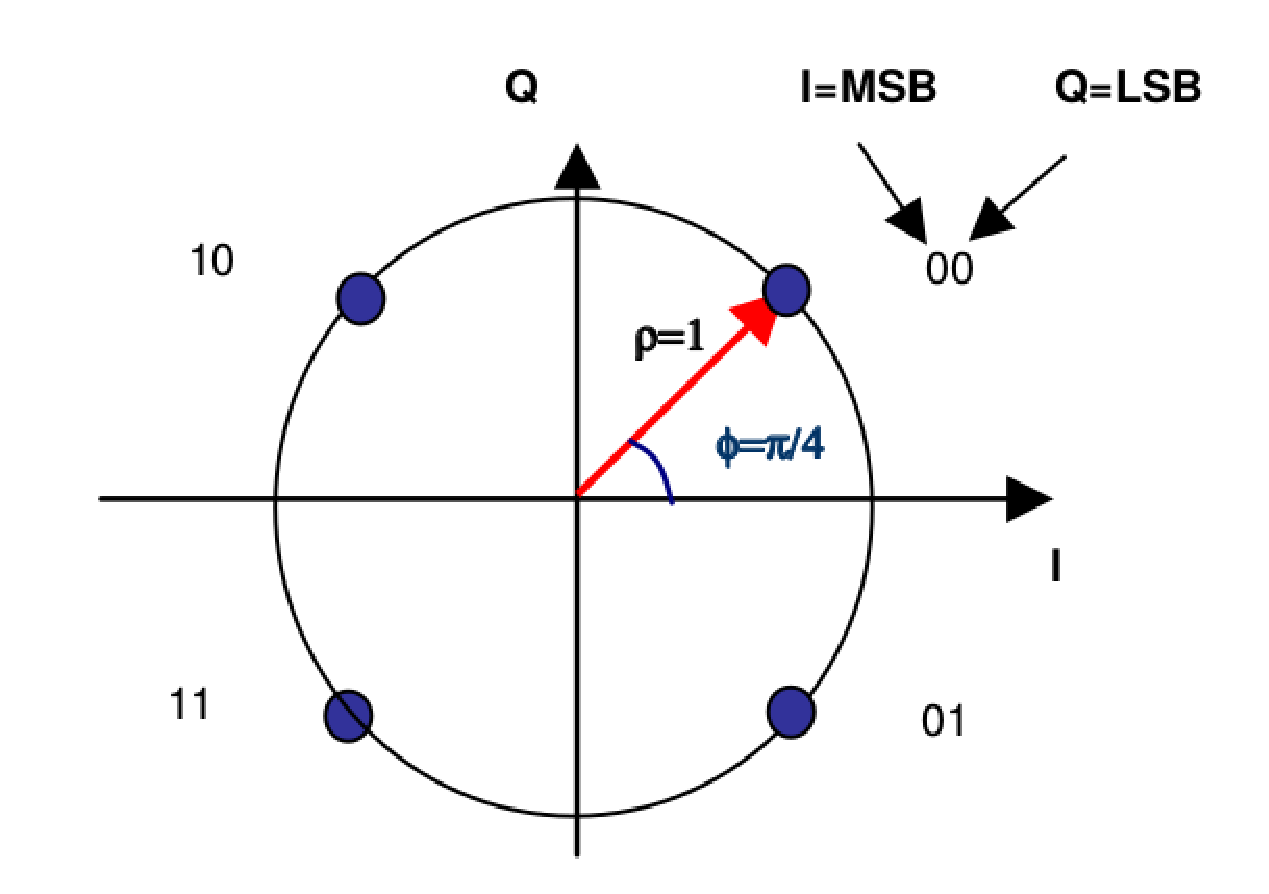
\includegraphics[width=\columnwidth]{./figs/qpsk}
\end{center}
\caption{Constellation diagram of QPSK}
\label{fig:qpsk}
\end{figure}
Fig. \ref{fig:qpsk} Shows the Constellation mapping for QPSK symbols.

\subsection{8PSK}
\begin{figure}[!ht]
\begin{center}
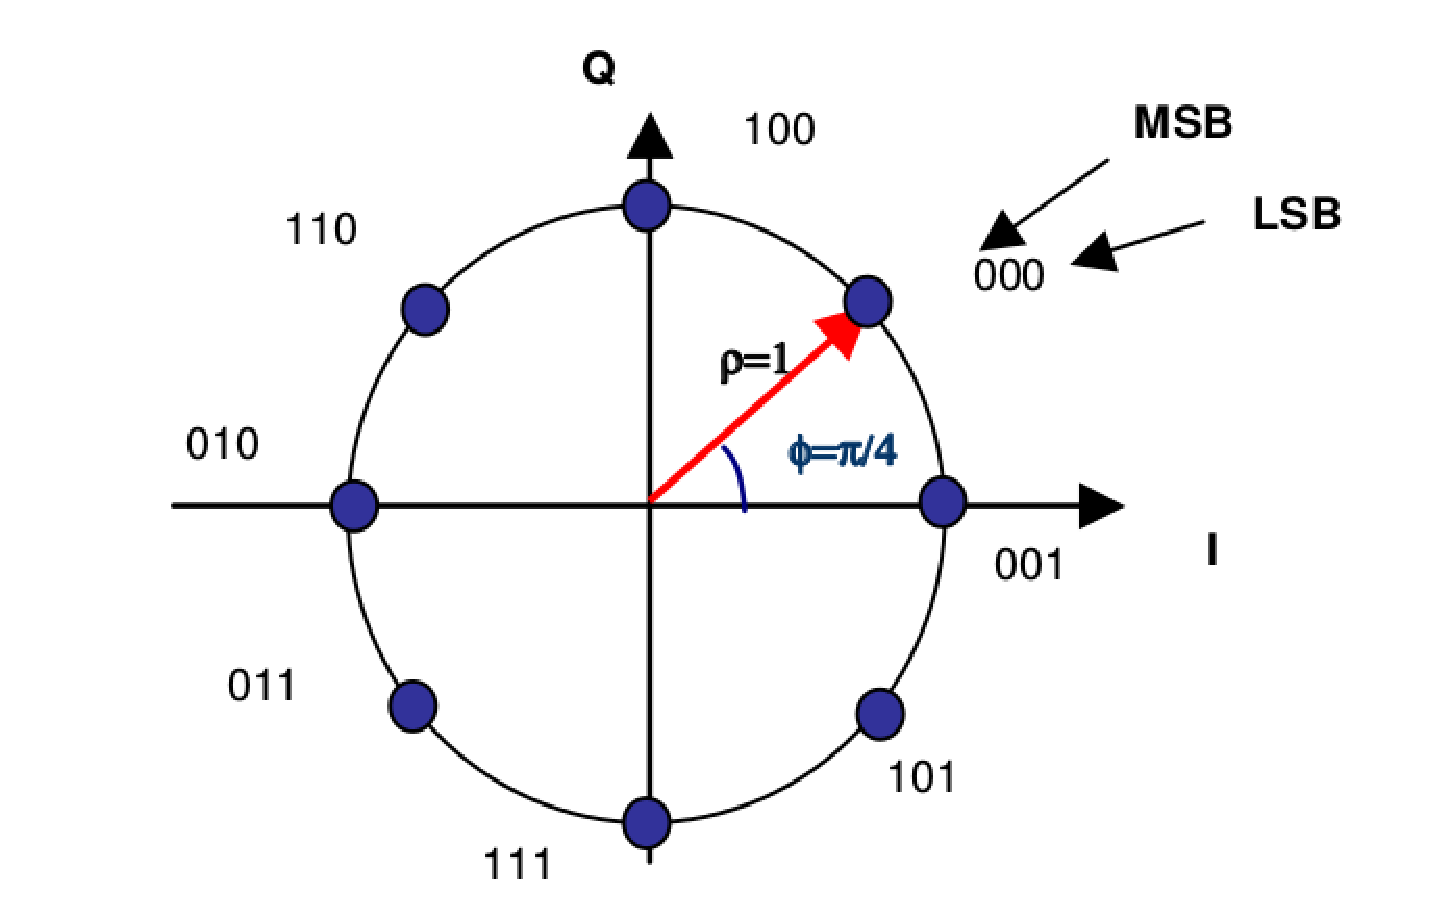
\includegraphics[width=\columnwidth]{./figs/8psk}
\end{center}
\caption{Constellation diagram of 8PSK}
\label{fig:8psk}
\end{figure}
Fig. \ref{fig:8psk} Shows the Constellation mapping for 8-PSK symbols.
\section{APSK}
\begin{equation}
Y=X+N
\end{equation}
\subsection{16-APSK}
\begin{equation}
X_n=
\begin{cases}
r_1 e^{j\brak{\phi_1+\frac{2\pi}{4}n}}& n=0,1,2,3\\
r_2 e^{j\brak{\phi_2+\frac{2\pi}{12}n}}& n=0,1,\dots,11
\end{cases}
\end{equation}
Where $\frac{r_2}{r_1}=2.6$,$\phi_1=45,\phi_2=15$
Fig. \ref{fig:16apsk} Shows the Constellation mapping for 16-APSK symbols.
%
\begin{figure}[!ht]
\begin{center}
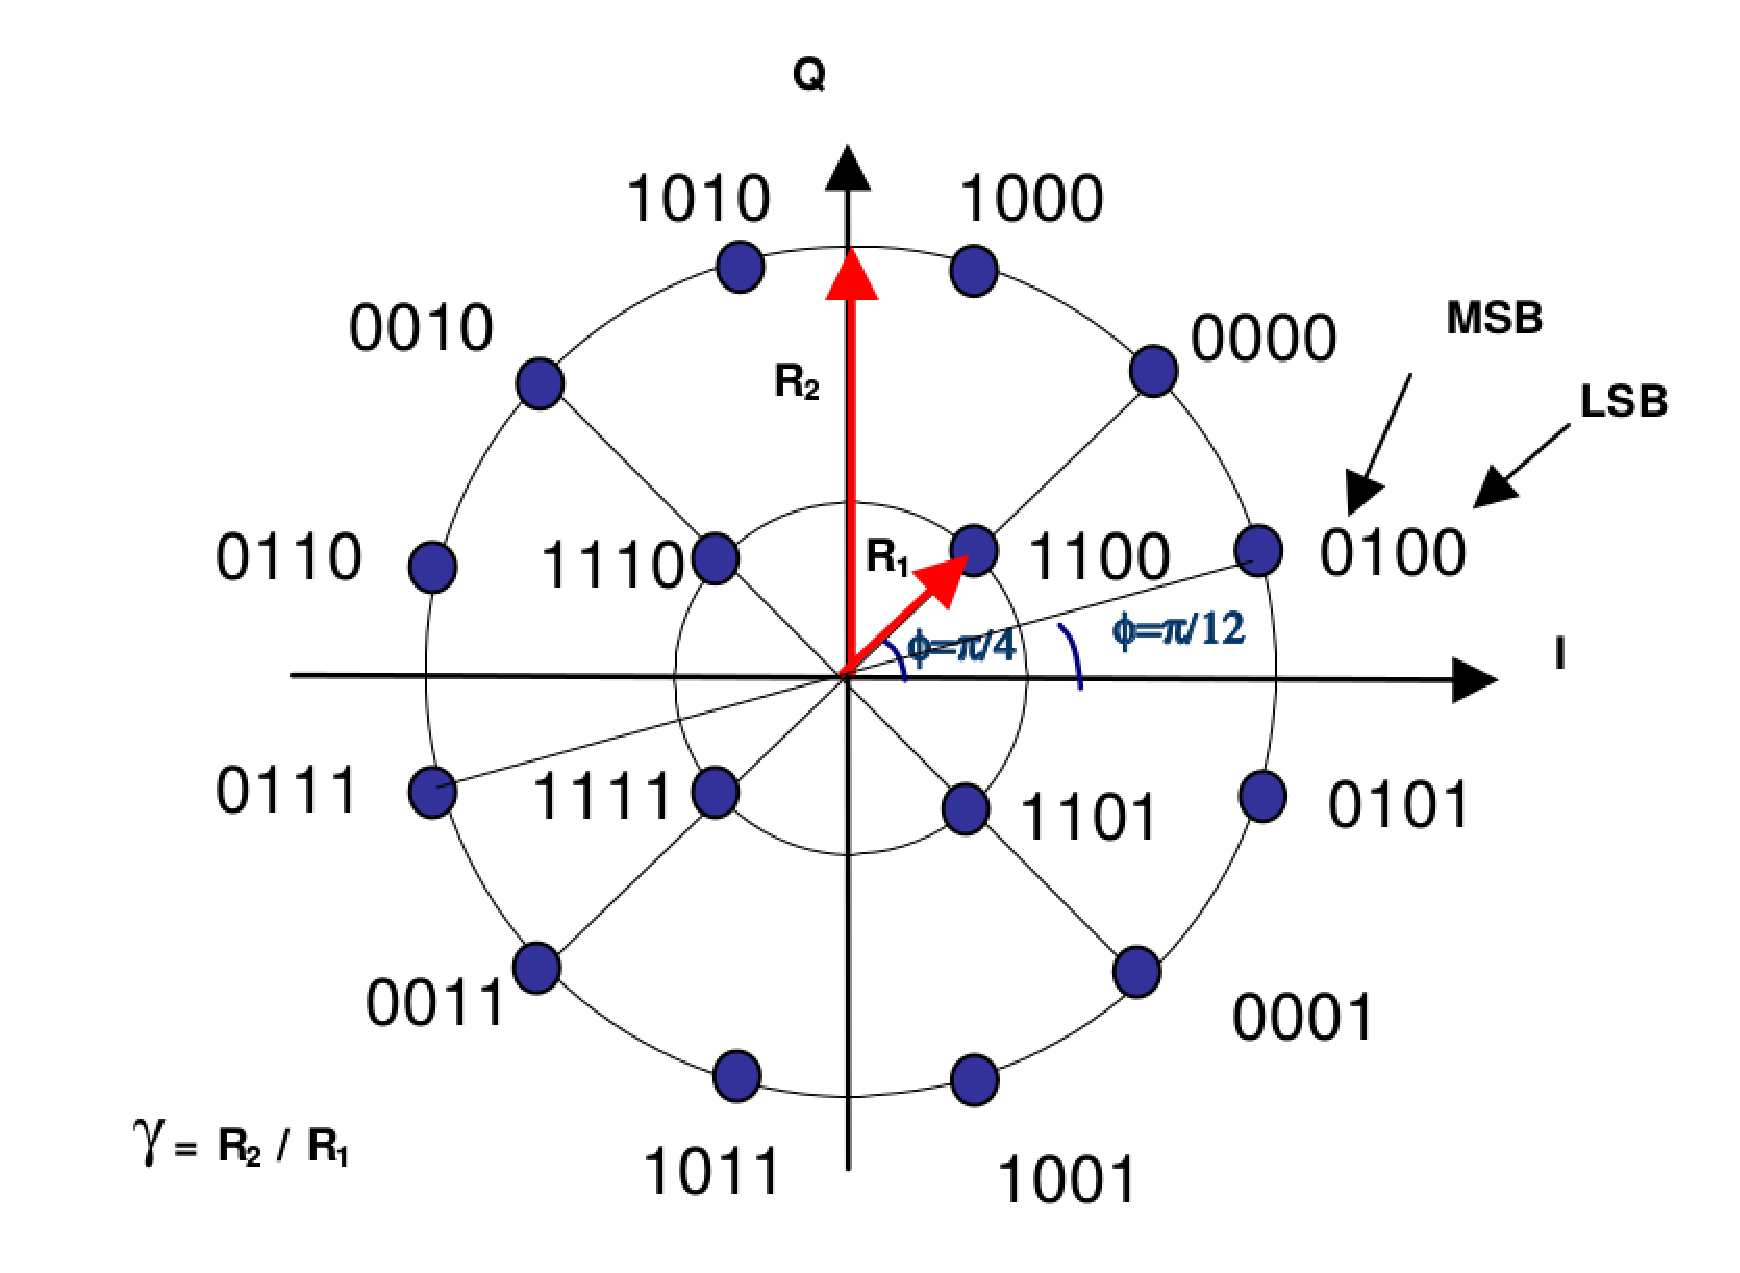
\includegraphics[width=\columnwidth]{./figs/16apsk}
\end{center}
\caption{Constellation diagram of 16APSK}
\label{fig:16apsk}
\end{figure}
%
\subsection{32-APSK}
\begin{equation}
X=
\begin{cases}
r_1 e^{j\brak{\phi_1+\frac{2\pi}{4}n}}& n=0,1,2,3\\
r_2 e^{j\brak{\phi_2+\frac{2\pi}{12}n}}& n=0,1,\dots,11\\
r_3 e^{j\brak{\phi_3+\frac{2\pi}{16}n}}& n=0,1,\dots,16
\end{cases}
\end{equation}
Where $\frac{r_2}{r_1}=2.54$,$\frac{r_3}{r_2}=4.33$,,$\phi_1=45,\phi_2=15,\phi_3=0$
Fig. \ref{fig:32apsk} Shows the Constellation mapping for 32-APSK symbols.
\begin{figure}[!ht]
\begin{center}
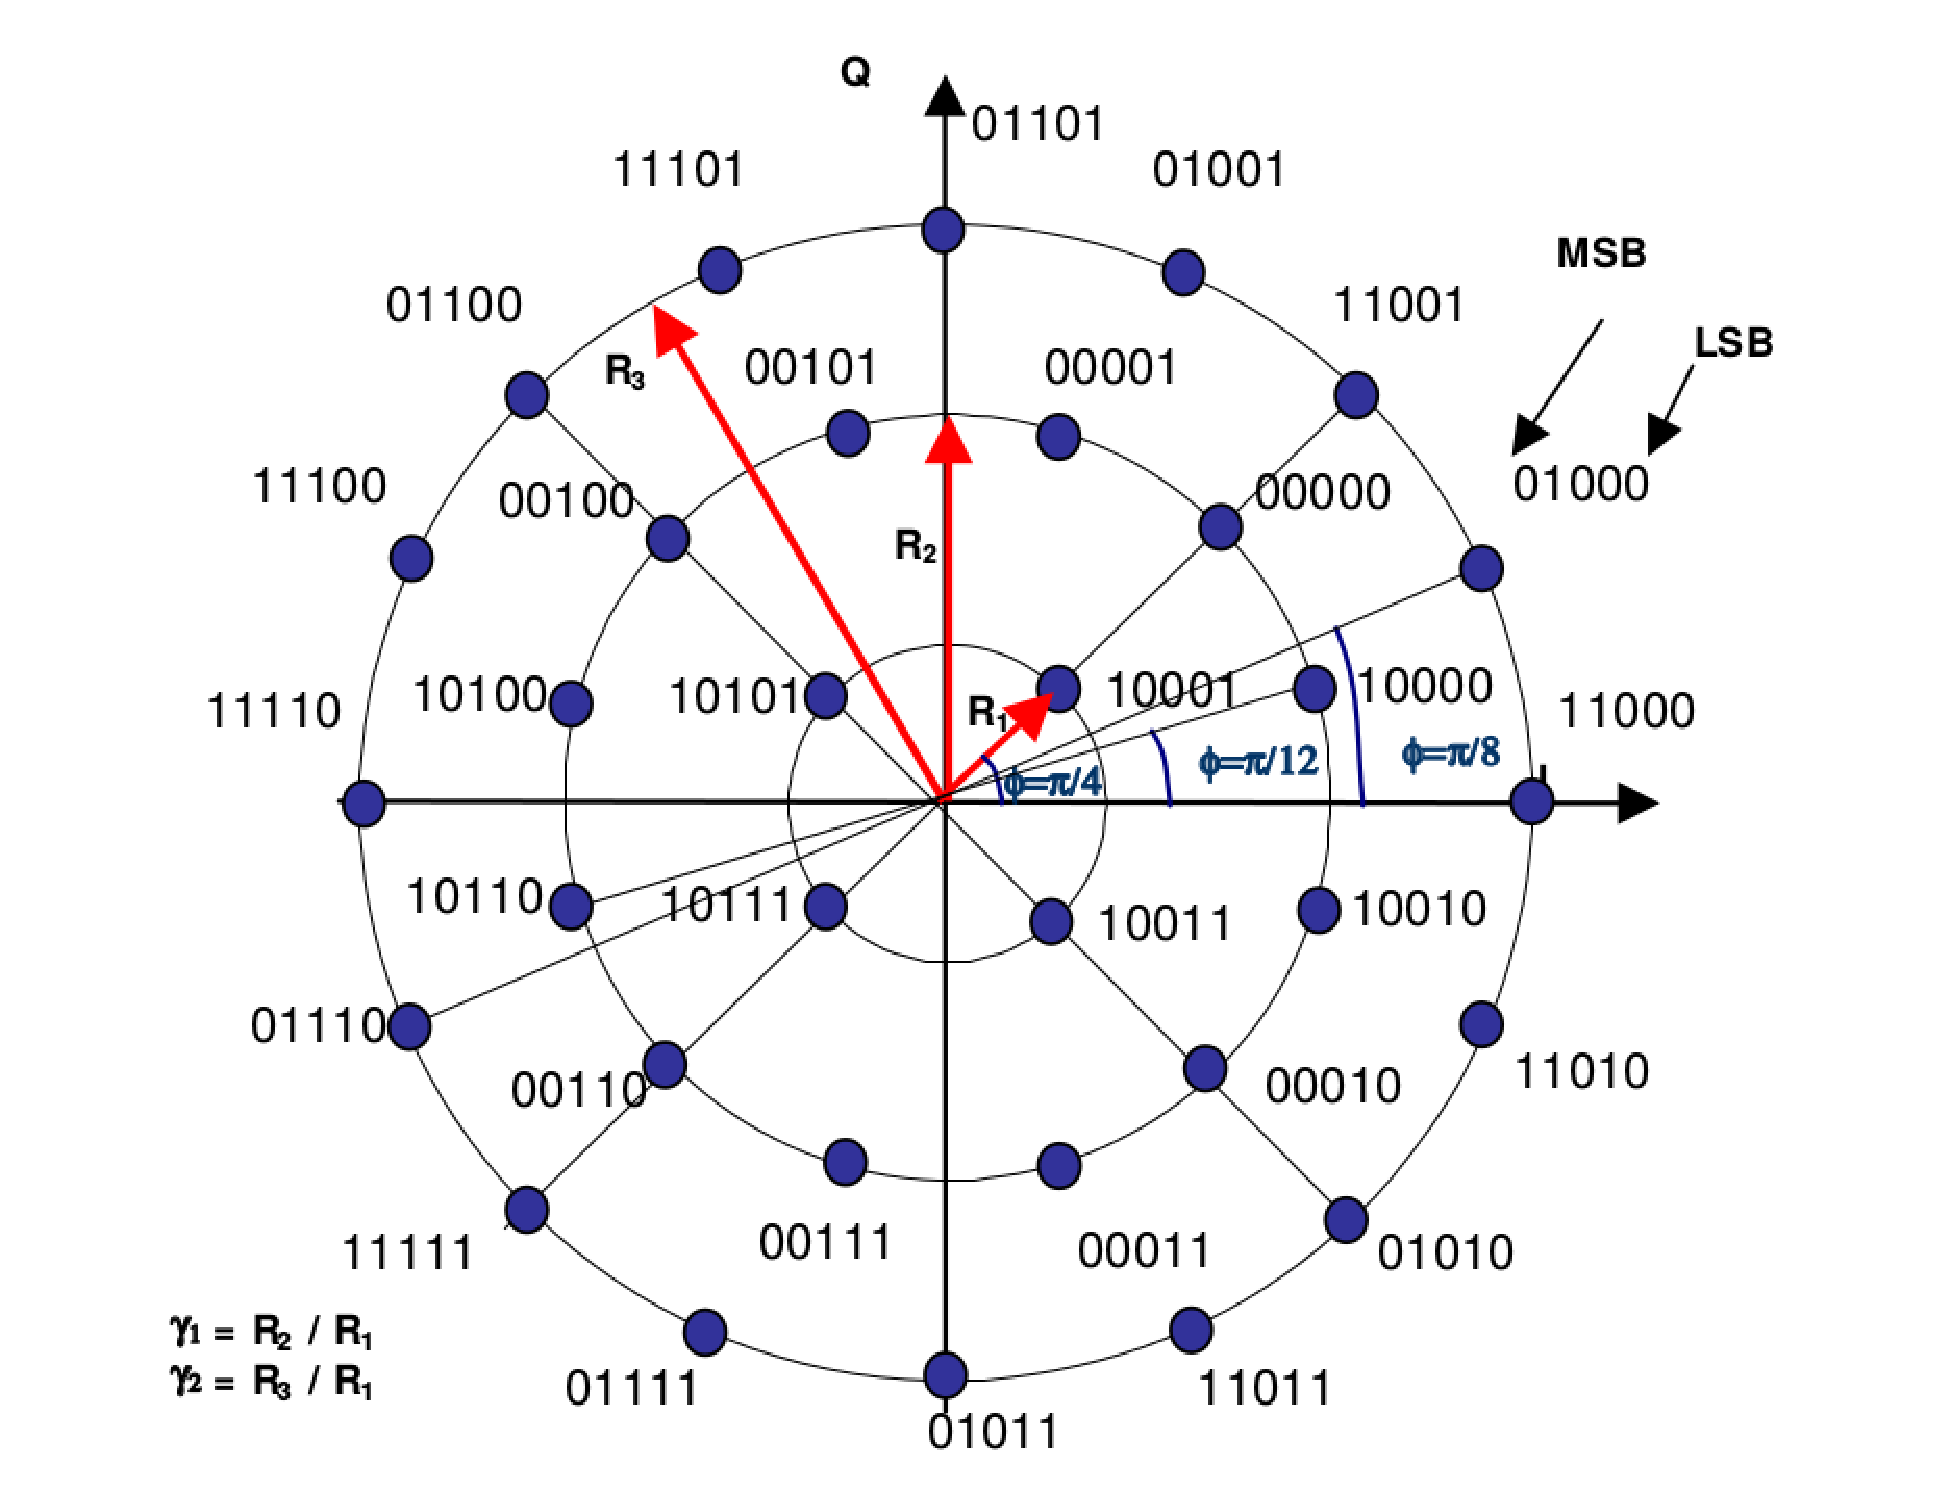
\includegraphics[width=\columnwidth]{./figs/32APSK}
\end{center}
\caption{Constellation diagram of 32APSK}
\label{fig:32apsk}
\end{figure}

\bibliography{IEEEabrv,mapping.bib}
\end{document}

